\documentclass[aspectratio=169,10pt]{beamer}

\usepackage{graphicx}
\usepackage{tikz}
\usetikzlibrary{positioning,arrows.meta}
\usepackage{xcolor}
\usepackage{booktabs}
\usepackage{tabularx}
\usepackage{array}
\usepackage{ragged2e}

\definecolor{GEUBlue}{RGB}{20,55,105}
\definecolor{GEULightBlue}{RGB}{238,244,251}
\definecolor{GEUGrey}{RGB}{90,90,90}
\definecolor{GEULightGrey}{RGB}{245,246,248}

\usetheme{default}
\setbeamertemplate{navigation symbols}{}
\setbeamertemplate{blocks}[rounded][shadow=false]
\setbeamersize{text margin left=5mm,text margin right=5mm}
\setbeamercolor{normal text}{fg=black,bg=white}
\setbeamercolor{frametitle}{fg=GEUBlue}
\setbeamercolor{structure}{fg=GEUBlue}
\setbeamercolor{block title}{fg=GEUBlue,bg=GEULightBlue}
\setbeamercolor{block body}{fg=black,bg=GEULightBlue}
\setbeamerfont{frametitle}{size=\large,series=\bfseries}

% Replace with the actual logo filename
\newcommand{\GEULogo}{graphicera_logo.jpeg}

% Header and footer
\setbeamertemplate{headline}{%
  \begin{tikzpicture}[remember picture,overlay]
    \node[anchor=north east,xshift=-0.25cm,yshift=-0.10cm]
      at (current page.north east)
      {\includegraphics[height=0.48cm]{\GEULogo}};
  \end{tikzpicture}
  \vspace{0.48cm}
}
\setbeamertemplate{frametitle}{%
  \vspace{0.01cm}
  \insertframetitle\par
  \vspace{0.02cm}
  \textcolor{GEUBlue}{\rule{\textwidth}{0.9pt}}
  \vspace{0.01cm}
}
\setbeamertemplate{footline}{%
  \leavevmode
  \hbox{%
  \begin{beamercolorbox}[wd=.82\paperwidth,ht=0.20cm,dp=0.05cm,leftskip=.3cm]{author in head/foot}
    \tiny Department of Computer Science \& Engineering | Graphic Era (Deemed to be University)
  \end{beamercolorbox}%
  \begin{beamercolorbox}[wd=.18\paperwidth,ht=0.20cm,dp=0.05cm,rightskip=.3cm]{date in head/foot}
    \hfill\tiny\insertframenumber/\inserttotalframenumber
  \end{beamercolorbox}}
}

\newcommand{\smallnote}[1]{\vspace{0.08cm}{\scriptsize\color{GEUGrey}#1}}
\newcommand{\placeholder}[1]{\textit{\color{GEUGrey}#1}}

\title{\textbf{Project-Based Learning}\\[2mm]\large Phase-I Evaluation}
\author{\textbf{Project Title}\\Team ID: XXXX}
\institute{Department of Computer Science \& Engineering\\Graphic Era (Deemed to be University), Dehradun}
\date{Academic Session 2026--27}

\begin{document}

% 1
\begin{frame}[plain]
\begin{tikzpicture}[remember picture,overlay]
\draw[GEUBlue,line width=3pt] (current page.north west) -- (current page.north east);
\node[anchor=north east,xshift=-0.45cm,yshift=-0.35cm] at (current page.north east)
{\includegraphics[height=1.0cm]{\GEULogo}};
\node[align=center,text width=.84\paperwidth] at ([yshift=.25cm]current page.center)
{{\color{GEUBlue}\fontsize{26}{30}\selectfont\bfseries PROJECT-BASED LEARNING}\\[3mm]
 {\fontsize{18}{22}\selectfont PHASE-I EVALUATION}\\[7mm]
 {\color{GEUGrey}\Large\bfseries Sangam - Your City Your Experience}\\[3mm]
 {\color{GEUBlue}\normalsize Team ID: DSCPP-III-2026-T059}};
\node[align=center,anchor=south,yshift=.42cm] at (current page.south)
{\bfseries Department of Computer Science \& Engineering\\
Graphic Era (Deemed to be University), Dehradun\\[-1mm]
\scriptsize Academic Session 2026--27};
\end{tikzpicture}
\end{frame}

% 2
\begin{frame}{Team \& Mentor Details}
\begin{columns}[T,totalwidth=\textwidth]
\column{.48\textwidth}
\begin{block}{Team Information}
\begin{tabular}{@{}ll@{}}
\textbf{Team ID:} & DSCPP-III-2026-T059\\
\textbf{Semester:} & 3rd \\
\textbf{Section:} & A , DS1, ML1\\
\textbf{Domain:} & \placeholder{Computer Science}
\end{tabular}
\end{block}
\column{.48\textwidth}
\begin{block}{Team Members}
1.\quad \placeholder{Srishti Dhasmana -- 2510010598}\\
2.\quad \placeholder{Ishita Bijalwan-- 2510380152}\\
3.\quad \placeholder{Nandini Rana -- 2510370024}\\

\end{block}
\end{columns}
\vspace{1mm}
\begin{block}{Mentor}
\placeholder{Mr.Manish Mehta}
\hfill
\textbf{Interactions completed: 4} 
\end{block}
\end{frame}

% 3
\begin{frame}{Problem Statement \& Motivation}
\begin{block}{Problem Statement}
\placeholder{Tourists visiting a new city often struggle to plan their visit efficiently, while most map and review platforms only show scattered lists of places with no real sense of order. This gap exists largely because route planning across multiple stops is a genuinely hard combinatorial problem, and most existing tools sidestep it rather than solve it. Our project aims to bridge this divide by helping users mark, browse, and organize places into a structured, optimized travel plan.}
\end{block}
\vspace{1mm}
\begin{columns}[T,totalwidth=\textwidth]
\column{.48\textwidth}
\textbf{\color{GEUBlue}Motivation}
\begin{itemize}\itemsep1pt
\item \placeholder{No structured way to plan a multi-stop visit.}
\item \placeholder{Existing apps show places, not usable routes.}
\item \placeholder{No efficient method to organize and search large place datasets.}
\end{itemize}
\column{.48\textwidth}
\textbf{\color{GEUBlue}Target Users / Stakeholders}
\begin{itemize}\itemsep1pt
\item \placeholder{Tourists and first-time visitors to a city.}
\item \placeholder{Hotels, restaurants, and attractions seeking visibility.}
\item \placeholder{Local guides and travel planners needing structured tools.}
\end{itemize}
\end{columns}
\end{frame}

% 4
\begin{frame}{Objectives}
\textbf{\color{GEUBlue}Project Objectives}
\vspace{1mm}
\begin{enumerate}\itemsep1pt
\item \placeholder{Develop a web-based solution to simplify city exploration and trip planning.}
\item \placeholder{Implement core features using C++ and DSA concepts.}
\item \placeholder{Apply DSA logic (graphs, searching, sorting) to structure routes and place data.}
\item \placeholder{Test the system for accuracy and performance.}
\item \placeholder{Demonstrate real-world use and future scope for expansion.}
\end{enumerate}
\vfill
\begin{center}
\colorbox{GEULightBlue}{\parbox{.80\textwidth}{\centering
\textbf{Key Objective:} \placeholder{"Enable users to mark places on a map and generate an optimized, structured travel plan, with measurable improvement in route efficiency over manual planning."}}}
\end{center}
\end{frame}

% 5
\begin{frame}{Proposed Solution}
\begin{columns}[T,totalwidth=\textwidth]
\column{.48\textwidth}
\textbf{\color{GEUBlue}Proposed Approach}
\begin{enumerate}\itemsep1pt
\item \placeholder{Input / Data Collection}
\item \placeholder{Processing / Core Algorithm}
\item \placeholder{System Logic}
\item \placeholder{Database / Storage}
\item \placeholder{Output / Visualization}
\end{enumerate}
\column{.48\textwidth}
\textbf{\color{GEUBlue}Key Features}
\begin{itemize}\itemsep1pt
\item \placeholder{Interactive Map with Place Markers}
\item \placeholder{Place Search and Autocomplete}
\item \placeholder{Route and Itinerary Optimization}
\item \placeholder{Category-based Browsing}
\item \placeholder{Route Visualization}
\end{itemize}
\end{columns}
\vfill
\smallnote{An interactive platform is designed to help tourists explore a city and plan visits using C++ and DSA concepts. User inputs such as selected places and preferences are collected and processed through efficient graph and search algorithms. The system logic computes optimized routes and handles edge cases such as unreachable or duplicate places, while structured data storage using vectors, hash tables, and graphs enables quick retrieval and scalability. Finally, a map-based visual output shows markers and computed routes, making trip planning intuitive, accessible, and efficient while reinforcing computational thinking.}
\end{frame}

% 6
\begin{frame}{Integration of PBL Course Concepts}
\scriptsize
\begin{center}
\renewcommand{\arraystretch}{1.25}
\begin{tabularx}{.96\textwidth}{@{}>{\bfseries}p{3.0cm}X p{2.5cm}@{}}
\toprule

Course & Concepts Applied & Project Module\\
\midrule
Data Structures in C &
\placeholder{Arrays, Linked Lists, Trees, Graphs, Hashing, etc.} &
Route Engine \& Place Lookup Module\\
OOPs with C++ &
\placeholder{Classes, Inheritance, Polymorphism, STL, etc.} &
Core Routing \& Itinerary Engine\\
\midrule
Web Design &
\placeholder{Styling, Navigation, User Interaction, Content} &
Website Frontend (HTML/CSS/JS + Map Integration)\\
\midrule
DBMS &
\placeholder{Tables, Normalization, Queries, CRUD Operations} &
Place \& Itinerary Storage Module\\
\bottomrule
\end{tabularx}
\end{center}
\end{tabularx}
\end{center}
\vfill
\begin{center}
\colorbox{GEULightBlue}{\parbox{.86\textwidth}{\centering
\textbf{Requirement:} Demonstrate meaningful integration of both subjects in \textbf{one} project.}}
\end{center}
\end{frame}

% 7
\begin{frame}{System Architecture / Workflow}
\begin{center}
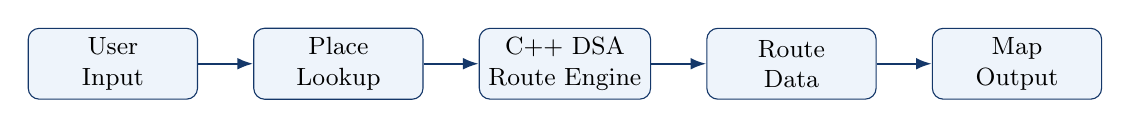
\begin{tikzpicture}[
node distance=7mm,
box/.style={rectangle,rounded corners,draw=GEUBlue,fill=GEULightBlue,
minimum width=2.15cm,minimum height=9mm,align=center,font=\small},
arrow/.style={-{Latex[length=2mm]},thick,draw=GEUBlue}
]
\node[box] (a) {User\\Input};
\node[box,right=of a] (b) {Place\\Lookup};
\node[box,right=of b] (c) {C++ DSA\\Route Engine};
\node[box,right=of c] (d) {Route\\Data};
\node[box,right=of d] (e) {Map\\Output};
\draw[arrow] (a)--(b); \draw[arrow] (b)--(c); \draw[arrow] (c)--(d); \draw[arrow] (d)--(e);
\end{tikzpicture}
\end{center}
\vspace{3mm}
\begin{columns}[T,totalwidth=\textwidth]
\column{.48\textwidth}
\textbf{\color{GEUBlue}Major Components}
\begin{itemize}\itemsep1pt
\item Website Frontend (HTML/CSS/JS + Map)
\item Database Module (Place \& Itinerary Storage)
\item C++ DSA Engine (Routing \& Search)
\end{itemize}
\column{.48\textwidth}
\textbf{\color{GEUBlue}Data / Control Flow}
\begin{itemize}\itemsep1pt
\item User marks places $\rightarrow$ website sends selection
\item Engine builds graph $\rightarrow$ places matched to nodes
\item C++ engine computes route, map displays result to user
\end{itemize}
\end{columns}
\end{frame}

% 8
\begin{frame}{Technology Stack \& Methodology}
\begin{columns}[T,totalwidth=\textwidth]
\column{.48\textwidth}
\begin{block}{Technology Stack}
\begin{itemize}\itemsep1pt
\item Programming: C++, HTML, CSS, JavaScript
\item Data Storage: SQLite (Lightweight DBMS)
\item Tools / Library: Leaflet.js (Map Rendering)
\item IDE: VS Code
\item Version Control: Git / GitHub
\end{itemize}
\end{block}
\column{.48\textwidth}
\begin{block}{Development Methodology}
\begin{enumerate}\itemsep1pt
\item Problem \& Requirement Analysis
\item Designing Graph Structure \& DSA Logic
\item Routing Engine \& Website Implementation
\item Route Accuracy Testing
\item Performance \& Usability Evaluation
\end{enumerate}
\end{block}
\end{columns}
\vfill
\begin{center}
\smallnote{Justify the selection of technologies and methodology.}
\end{center}
\end{frame}

% 9
\begin{frame}{Initial Progress \& Team Contribution}
\begin{columns}[T,totalwidth=\textwidth]
\column{.44\textwidth}
\textbf{\color{GEUBlue}Progress Achieved}
\begin{itemize}\itemsep1pt
\item Background / literature study on existing map \& trip-planning tools
\item Requirements identified (place data, route optimization)
\item System architecture \& workflow designed
\item Website skeleton (HTML/CSS/JS + map) implemented
\item DSA logic planned for graph structuring \& routing
\end{itemize}
\column{.52\textwidth}
\textbf{\color{GEUBlue}Individual Contribution}
\vspace{1mm}
\scriptsize
\begin{tabularx}{\textwidth}{@{}p{1.8cm}p{2.0cm}X@{}}
\toprule
Member & Role & Contribution\\
\midrule
M1 & Frontend \& Search Logic & HTML/CSS/JS interface, map integration; implemented trie-based search and hash table lookup in C++\\
M2 & Core DSA \& Routing & Graph construction, Dijkstra/A* implementation, itinerary optimization logic in C++\\
M3 & Database \& Data Structuring & SQLite schema and persistence layer; structured place data using vectors and linked lists in C++\\
\bottomrule
\end{tabularx}
\end{columns}
\end{frame}


% 10
\begin{frame}{Roadmap, Expected Outcomes \& References}
\begin{columns}[T,totalwidth=\textwidth]
\column{.47\textwidth}
\textbf{\color{GEUBlue}Roadmap}
\begin{enumerate}\itemsep1pt
\item Phase-I: Proposal \& Design
\item Phase-II: Development
\item Phase-III: Final Implementation
\end{enumerate}
\vspace{1mm}
\textbf{\color{GEUBlue}Expected Outcomes}
\begin{itemize}\itemsep1pt
\item Working city guide platform with interactive map \& itinerary planner
\item Functional route optimization across multiple selected places
\item Faster, more efficient trip planning for tourists
\item Scope to expand dataset \& add more cities
\end{itemize}
\column{.47\textwidth}
\textbf{\color{GEUBlue}References}
\begin{enumerate}\itemsep1pt
\item E. W. Dijkstra, "A Note on Two Problems in Connexion with Graphs," Numerische Mathematik, 1959
\item P. Hart, N. Nilsson, B. Raphael, "A Formal Basis for the Heuristic Determination of Minimum Cost Paths," IEEE Trans. SSC, 1968
\item OpenStreetMap contributors -- openstreetmap.org
\item Leaflet.js documentation -- leafletjs.com
\end{enumerate}
\vfill
\begin{center}
\colorbox{GEUBlue}{\parbox{.78\textwidth}{\centering\color{white}\textbf{Thank You}\\Questions \& Suggestions}}
\end{center}
\end{columns}
\end{frame}

\end{document}
